\usetikzlibrary{arrows}
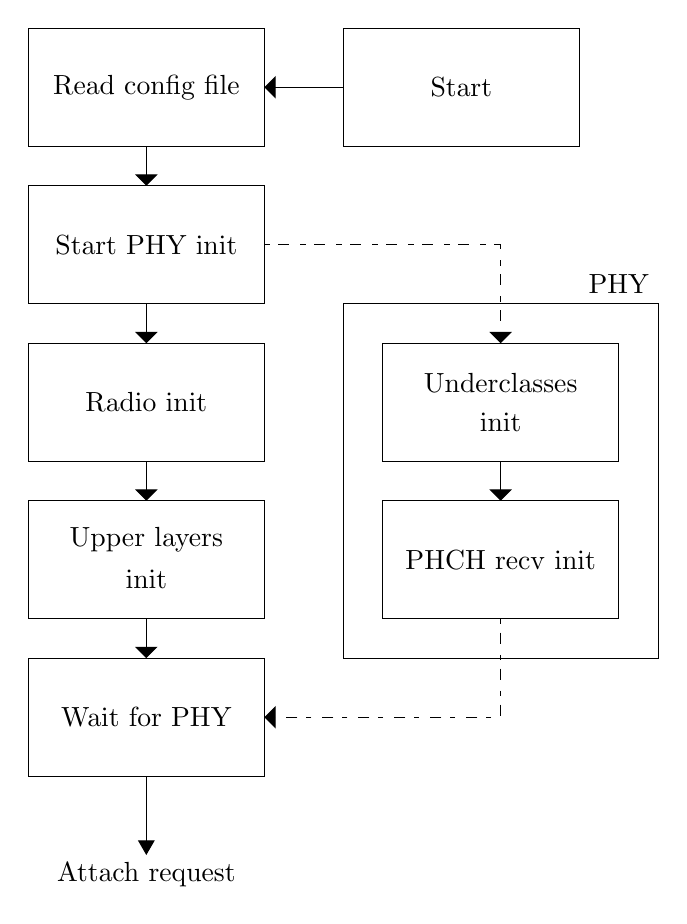
\begin{tikzpicture}


\draw  (-4,3) rectangle (-1,1.5);
\draw  (-8,3) rectangle (-5,1.5);
\draw  (-8,1) rectangle (-5,-0.5);
\draw  (-8,-1) rectangle (-5,-2.5);
\draw  (-8,-3) rectangle (-5,-4.5);
\draw  (-3.5,-1) rectangle (-0.5,-2.5);
\draw  (-3.5,-3) rectangle (-0.5,-4.5);
\draw  (-8,-5) rectangle (-5,-6.5);
\draw  (-4,-0.5) rectangle (0,-5);

\draw [-triangle 90](-4,2.25) -- (-5,2.25);
\draw [-triangle 90](-6.5,1.5) -- (-6.5,1);
\draw [-triangle 90](-6.5,-0.5) -- (-6.5,-1);
\draw [-triangle 90](-6.5,-2.5) -- (-6.5,-3);
\draw [-triangle 90](-6.5,-4.5) -- (-6.5,-5);
\draw [dash pattern=on 2pt off 3pt on 4pt off 4pt][-triangle 90](-5,0.25) -- (-2,0.25) -- (-2,-1);
\draw [dash pattern=on 2pt off 3pt on 4pt off 4pt][-triangle 90](-2,-4.5) -- (-2,-5.75) -- (-5,-5.75);
\draw [-triangle 90](-2,-2.5) -- (-2,-3);

\node at (-2.5,2.25) {Start};
\node at (-6.5,2.25) {Read config file};
\node at (-6.5,0.25) {Start PHY init};
\node at (-6.5,-1.75) {Radio init};
\node at (-6.5,-3.5) {Upper layers};
\node at (-6.5,-5.75) {Wait for PHY};
\node at (-2,-1.5) {Underclasses};
\node at (-2,-3.75) {PHCH recv init};
\draw [-triangle 60](-6.5,-6.5) -- (-6.5,-7.5);
\node at (-6.5,-7.75) {Attach request};
\node at (-0.50,-0.25) {PHY};
\node at (-6.5,-4) {init};
\node at (-2,-2) {init};
\end{tikzpicture}